\chapter{外文翻译}

{
  \setlength{\parindent}{0em}

  文献原文:

  Zhang X, Luo H, Fan X, et al. AlignedReID: Surpassing Human-Level Performance in Person Re-Identification, 2017. \par

}

\vspace{2em}

{
  \renewcommand{\cleardoublepage}{}
  \renewcommand{\clearpage}{}
  \titleformat{\chapter}[block]{\sanhao\songti\bfseries\filcenter}{}{0em}{}{}
  \chapter*{对齐再识别:超越人类的表现}
}

\section*{摘要}

在这篇论文中,我们提出了一种全新的方法,叫做对齐再识别。最终部署时只使用全局特征,全局特征的鉴别能力是通过与局部特征的共同学习获得的。在共同学习的过程中,局部特征通过计算最短路径对齐和匹配不同人体区域,不需要额外的监督信息。在学习完成之后,我们只使用全局特征计算图像的相似度,进行检索。我们的方法在Market1501数据集上获得了94.0\%的rank-1准确率,在CUHK03上获得了96.1\%的rank-1准确率,均比目前最好的方法提升了很多。我们也评估了人类所能达到的极限,发现我们的方法首次在两个公开数据集上超过了人类表现!

\section{介绍}

行人再识别,是计算机视觉中的一个子任务,目标是在不同的时空鉴别出目标行人。他应用广泛,从跨摄像头跟踪,到销售商店客流量分析,均可发挥巨大作用。同很多视觉任务一样,再识别的难点也在于视角,光照的变化和遮挡的存在。
传统的方法通常在底层特征上着力。但自从深度学习复兴之后,卷积神经网络成为了这一难题的主流方法,通过端到端的特征学习,以及丰富的度量学习损失函数设计(比如对比损失,三元损失,四元损失和难样本挖掘三元损失),这一方法达到了前所未有的准确率。
很多卷积神经网络的方法仅仅考虑学习全局特征,而忽略了行人的空间结构。这些方法主要有以下缺点:
\begin{enumerate}
\item 不准确的行人检测会影响特征学习。
\item 行人被遮挡时,全局特征会引入无关的背景信息。
\item 视角变化和非刚性物体的形变使度量学习更加困难。
\item 外观相似但并非同一人的情况大量存在,这时候需要突出局部特征才能鉴别出这类行人。
\end{enumerate}
为了解决上述问题,近期的一些工作在划分人体区域学习局部特征上着手,但是仍然无法解决检测不准确、姿态变化、遮挡等难题。也有研究者从姿态估计着手,但是这种方法需要额外的监督信息,同时在姿态估计的步骤中往往更容易发生错误。
在本文中,我们提出了一种全新的对齐再识别的方法,虽然也是学习全局特征。但是在学习的过程中使用局部特征对齐协同学习,不需要额外的监督信息或者显式的姿态估计。在学习阶段,我们有两条支路分别学习局部特征和全局特征。在局部特征支路,我们引入了最短路径损失。在部署使用阶段,我们只使用全局特征。因为我们发现只使用全局特征已经和多种特征融合的效果同样好!这从另一方面说明,在协同训练的过程中,局部特征帮助全局特征变得更有鉴别能力。同时简洁的全局特征使得我们的方法便于部署到大尺度行人再识别系统中。

\section{方法} 

\subsection{对齐再识别} 

对于每张输入图片,我们使用Resnet50提取特征,得到2048X7X7的特征图,然后使用全局池化得到2048维的全局特征。对于局部特征我们首先使用使用垂直方向的池化得到2048X7的特征图,然后使用动态匹配局部区域,得到最小距离,作为局部特征之间的距离度量。这样的特征提取方式隐含着人在图片中通常直立的假设。
给定两幅图片的局部特征,在我们的实验中H为7,即行人从头到脚被分为7个部分。我们首先计算两两之间的距离矩阵:
\begin{equation} {d_{i,j}} = \frac{{{e^{\|{f_i} - {g_j}\|{_2}}} - 1}}{{{e^{\|{f_i} - {g_j}\|{_2}}} + 1}}\qquad i,j \in 1,2,3, \cdots ,H \end{equation}

采用这样形式的变换的原因是:改距离可以归一化到[0,1]之间。然后定义局部特征时间的距离为距离矩阵D中,从(1,1)到(H,H)之间的最短路径。改最短路可以由动态规划计算得到。如图1所示,图像A和图像B是同一行人的不同视角的图片。身体不同部分的对齐,比如图A的第一部分和图B的第4部分,在最短路径的第一个转折中体现出来。同时,也存在一些不对应部分的对齐,比如图A的第一部分和图B的第一部分。我们认为,不对应部分的对齐是有助于维护垂直对齐的顺序的。不对应部分有着更大的L2距离,梯度更接近于0,英尺这些对齐在最短路中贡献可以忽略。因此最短路的总距离主要由对应部分的对齐决定。

\begin{figure}[!htbp]
\centering
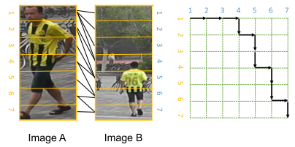
\includegraphics[width=.45\linewidth,keepaspectratio]{data/waiwenfanyi/placeholder.png}
\caption{图像A和图像B是同一行人的不同视角的图片。身体不同部分的对齐,比如图A的第一部分和图B的第4部分,在最短路径的第一个转折中体现出来。}
\label{figure:placeholder}
\end{figure}

全局和局部特征共同定义了图像在学习阶段的距离。我们选择TriHard损失作为度量损失函数。对于每一个样本,我们会根据全局特征之间的距离选取最有竞争力的样本对,获得3元组。而三元组的损失则是根据全局特征距离和局部特征距离共同计算的。这样做的原因出于两点考虑:1. 全局距离的计算更加快;2. 我们观察到使用全局距离和局部距离作为难样本挖掘的手段,没有很大的差别。

\subsection{Mutual Learning应用于度量学习}

我们将mutual learning应用于对齐再识别中,来进一步提升效果。在知识蒸馏一文中,作者使用小的学生网络学习大的教师网络中的知识。他的工作用于分类任务中,与他的工作不同,我们采用矩阵级别的均方误差作为新提出的相互学习损失,用于度量学习的任务中。

总体的损失由度量损失、分类损失、分类相互学习损失和度量相互学习损失构成。其中,度量损失是由局部和全局特征距离共同决定的,但是度量相互损失仅由全局特征距离决定。
下面介绍度量相互损失的实现:给定一个batch的图片,可以使用全局特征计算出距离矩阵。使用ResNet50和Resnet50-Xception作为基础骨架模型,得到两个不同的学生模型。使用距离矩阵的均方误差作为损失函数,使得两个学生相互学习。在实践中,我们发现使用停止梯度的操作可以加快收敛。即停止Resnet50学生网络的梯度更新,将其作为常数,使得Resnet50-Xception学生逼近Resnet50,以及用相同的方式让Resnet50逼近Resnet50-Xception。

\section{实验}

\subsection{数据集}

Market1501数据集包含32668张图像,1501个行人,6个摄像视角。训练集中有750个行人,测试集中有751个行人。与提出数据集的作者相同,我们也将mAP作为我们的指标的一种。

CUHK03包含13164张图片,1360个行人,他同时提供了DPM检测器检测的行人和手工标注的行人。

MARS数据集是Market1501的扩展版本,所有的行人都是自动检测的。因此可能包含一些虚警增加难度,同时每个ID可能包含多余1个候选答案。他包含20478个tracklet和1261个行人,6个拍摄视角。

CUHK-SYSU是一个大尺度行人搜索的数据集,包含18184张图片,每张图中含有多个行人,共计99809个行人检测框,8432个行人。

注意我们使用全部数据集的样例训练单个模型,对于MARS、CUHK-SYSU和Market1501数据集我们使用官方的训练和评估协议。但是在CUHK03上,由于我们使用了全部benchmark的数据集训练了一个模型,和官方的测试方式(随机划分数据集为训练集和测试集,测试包含100个行人,重复20次)有些不同。因此,我们仅仅随机划分数据集一次,训练集与其他数据集的训练集一同作为整个模型的训练集,将测试集作为CUHK03上衡量CUHK03数据集性能的测试集。由于我们划分的测试集含有200个行人,可以认为这个评估协议比原始的协议更具有挑战性。

\subsection{实现细节}

我们使用Resnet50和Resnet50-Xception制品为基础模型。输入图片缩放到224X224。数据增强使用随机水平翻转和随机截取。TriHard损失的margin设为0.3,mini-batch设为128,在一个batch中确保每个id的图片有4张。每个epoch包含2000个mini-batch。我们采用adam优化器,初始学习率设为0.001,在第80和第160个epoch时,衰减0.1训练至收敛。
对于对偶学习,相互分类损失的权重设为0.01,相互度量损失的权重设为0.001,使用adam优化器。初始学习率设为0.0003,分别在60和120epochs时衰减到0.0001和0.00001。

\subsection{对齐再识别的优点}

我们首先定性分析对齐的效果。在图2的(a)中,由于右边行人的检测不准确,两张原始图片原本无法对齐。对齐再识别算法将左边第一部分和右边的上上个部分匹配在一起,实现了对齐。在(d)中两个行人外观相似,但属于不同id,右边行人衣服上的标志找在左边找不到相似的部分,因此最短路中对应部分的路径也变得更长。

\begin{figure}[!htbp]
\centering
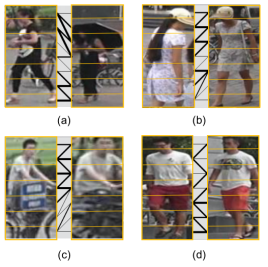
\includegraphics[width=.35\linewidth,keepaspectratio]{data/waiwenfanyi/fig2.png}
\caption{黑色线条表示两个新人局部的对齐:加粗表示对最短路贡献大。在(a-c)中行人有着相同的id,而在(d)中行人有着不同的id。}
\label{figure:fig2}
\end{figure}

然后我们将对齐再识别与基准模型对比。基准模型没有使用局部特征支路。两个结果使用相同的网络和训练参数设置。我们观察到对齐再识别方法能提升3.5\%到6.0\%的rank-1指标和5.0\%到8.4\%的mAP指标。
我们发现将局部特征和全局特征放在一起,rank-1指标只进一步提升了0.3\%到0.5\%,但该方法会变得更加耗时,因此我们推荐只是用全局特征。

\subsection{与其他最新方法比较}

在Market1501数据集上,使用rerank的GLAD达到了89.9\%的rank-1指标和81.1\%的mAP。而我们的对齐再识别在没有使用rerank的情况下就达到了92.6\%的rank-1指标和82.3\%的mAP。如果使用rerank,则进一步提升到94\%和91.2\%

在CUHK03数据集上,在不使用rerank的情况下HydraPlus-Net获得了91.8\%的rank1,而我们的对齐再识别为91.9\%。再次强调,我们的测试候选集为200张,我们的测试协议更加困难。同时在使用rerank的情况下,我们的方法获得了96.1\%的rank-1。

\begin{figure}[!htbp]
  \centering
  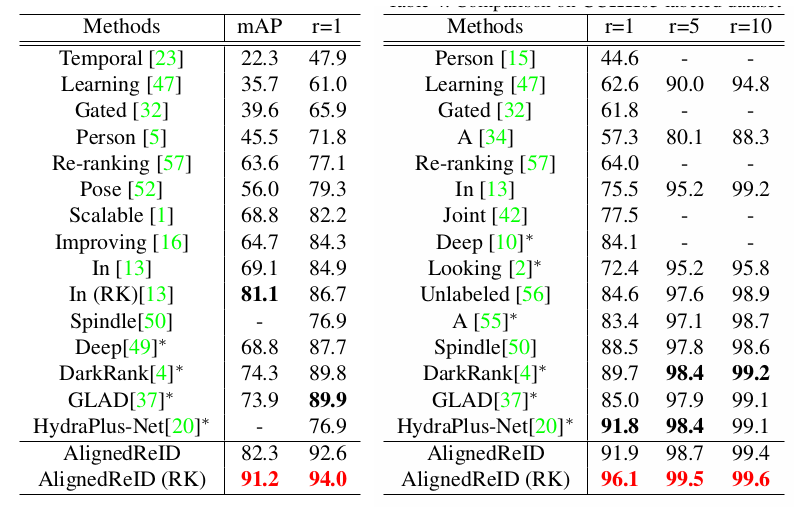
\includegraphics[width=.85\linewidth,keepaspectratio]{data/waiwenfanyi/compare.png}
  \caption{左图:在Market1501数据集上的性能比较,右图:在CUHK03数据集上的性能比较}
  \label{figure:compare}
\end{figure}

\subsection{总结}
在这篇文章中,我们阐明了隐式局部特征对齐对提升全局特征学习的巨大作用。这一惊奇的结果给予了我们重要启发:1). 端到端的学习需要结构先验,否则就是盲学。2). 尽管我们的方法在Market1501和cuhk03数据集上超过了人类的表现,但是机器想要在更广泛的领域战胜人类仍然有很长的路要走,比如在验证集中我们发现了一些低级的错误。

\begin{figure}[!htbp]
  \centering
  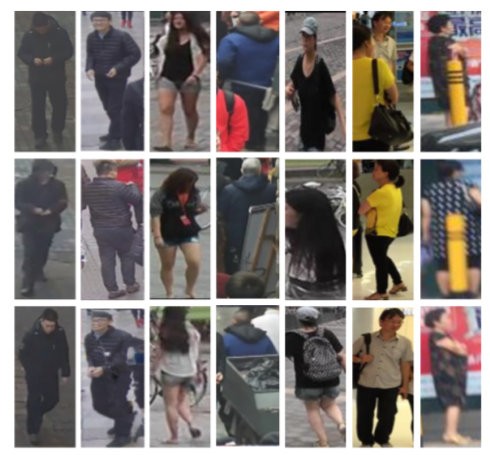
\includegraphics[width=.4\linewidth,keepaspectratio]{data/waiwenfanyi/bad.png}
  \caption{在验证集中发现的一些低级错误}
  \label{figure:bad}
\end{figure}
